  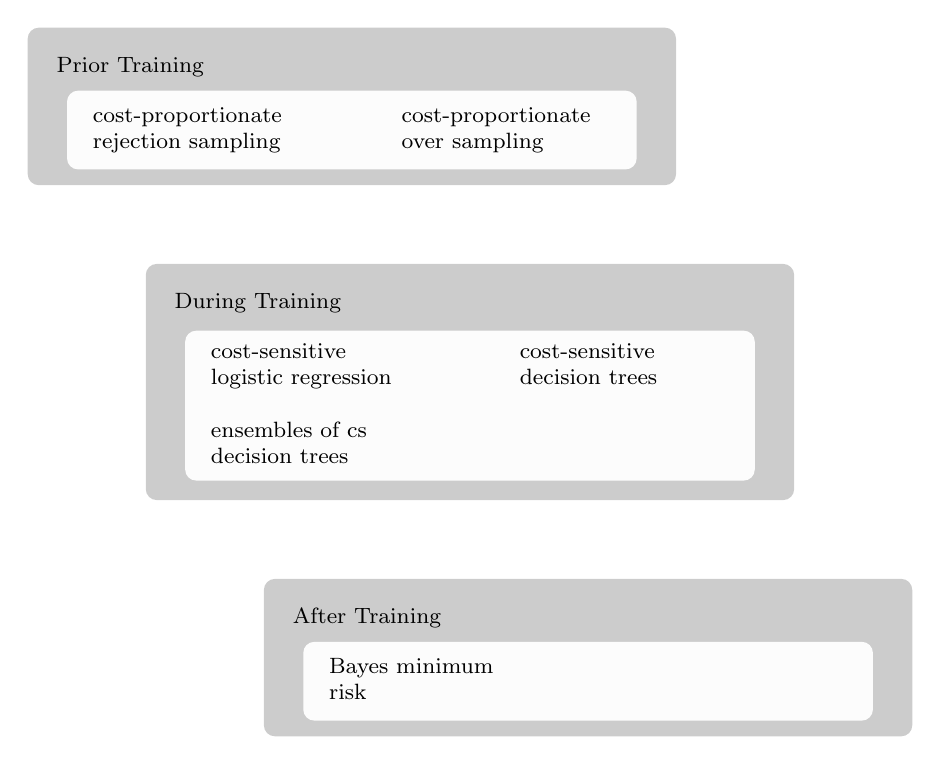
\begin{tikzpicture}[node distance=2.5cm]
  \tikzstyle{every node}=[font=\footnotesize]
  
  % Main boxes
  \node (data1) [rectangle, rounded corners, minimum width=2cm, minimum height=2cm,text 
                centered, fill=black!20, text width=8cm] 
                {\tabular{p{7.5cm}} Prior Training\\ \\ \\ \\ \endtabular};
  \node (data2) [rectangle, rounded corners, minimum width=2cm, minimum height=3cm,text 
                centered, fill=black!20, right of=data1, yshift=-3.5cm, xshift=-1cm, text 
                width=8cm] {\tabular{p{7.5cm}} During Training\\ \\ \\ \\ \\ \\ \\ \endtabular};
  \node (data3) [rectangle, rounded corners, minimum width=2cm, minimum height=2cm,text 
                centered, fill=black!20, right of=data2, yshift=-3.5cm, xshift=-1cm, text 
                width=8cm] {\tabular{p{7.5cm}} After Training\\ \\ \\ \\  \endtabular};

  \node (data11) [rectangle, rounded corners, minimum width=2cm, minimum height=1cm, 
                fill=black!1, below of=data1, yshift=2.2cm, text width=7cm]
                {\tabular{p{3.5cm} p{3.5cm}} cost-proportionate & cost-proportionate \\ 
                rejection sampling & over sampling \endtabular};

  \node (data21) [rectangle, rounded corners, minimum width=2cm, minimum height=1cm, 
                fill=black!1, below of=data2, yshift=2.2cm, text width=7cm]
                {\tabular{p{3.5cm} p{3.5cm}} cost-sensitive & cost-sensitive \\ 
                logistic regression & decision trees \\ \\ 
                ensembles of cs & \\ decision trees & \\ \endtabular};
  
  \node (data31) [rectangle, rounded corners, minimum width=2cm, minimum height=1cm, 
                fill=black!1, below of=data3, yshift=2.2cm, text width=7cm]
                {\tabular{l} Bayes minimum\\ risk  \endtabular};
	
	% Arrows
% 	\draw[thick,->,>=stealth] (data1) to (data2);
%   \draw[thick,->,>=stealth] (data2) to (data3);
  \end{tikzpicture}
 
%  \tikzstyle{startstop} = [rectangle, rounded corners, minimum width=2cm, minimum height=4cm,text 
% centered, draw=black, fill=black!20]
% \tikzstyle{startstop2} = [rectangle, rounded corners, minimum width=2cm, minimum height=1cm,text 
% centered, draw=black, fill=black!20]
% \tikzstyle{startstop3} = [rectangle, rounded corners, minimum width=2cm, minimum height=2.9cm,text 
% left, draw=black, fill=black!1]
% \tikzstyle{arrow} = [thick,->,>=stealth]